\documentclass[12pt,fleqn]{article}\usepackage[]{graphicx}\usepackage[]{color}
%% maxwidth is the original width if it is less than linewidth
%% otherwise use linewidth (to make sure the graphics do not exceed the margin)
\makeatletter
\def\maxwidth{ %
  \ifdim\Gin@nat@width>\linewidth
    \linewidth
  \else
    \Gin@nat@width
  \fi
}
\makeatother

\definecolor{fgcolor}{rgb}{0.345, 0.345, 0.345}
\newcommand{\hlnum}[1]{\textcolor[rgb]{0.686,0.059,0.569}{#1}}%
\newcommand{\hlstr}[1]{\textcolor[rgb]{0.192,0.494,0.8}{#1}}%
\newcommand{\hlcom}[1]{\textcolor[rgb]{0.678,0.584,0.686}{\textit{#1}}}%
\newcommand{\hlopt}[1]{\textcolor[rgb]{0,0,0}{#1}}%
\newcommand{\hlstd}[1]{\textcolor[rgb]{0.345,0.345,0.345}{#1}}%
\newcommand{\hlkwa}[1]{\textcolor[rgb]{0.161,0.373,0.58}{\textbf{#1}}}%
\newcommand{\hlkwb}[1]{\textcolor[rgb]{0.69,0.353,0.396}{#1}}%
\newcommand{\hlkwc}[1]{\textcolor[rgb]{0.333,0.667,0.333}{#1}}%
\newcommand{\hlkwd}[1]{\textcolor[rgb]{0.737,0.353,0.396}{\textbf{#1}}}%
\let\hlipl\hlkwb

\usepackage{framed}
\makeatletter
\newenvironment{kframe}{%
 \def\at@end@of@kframe{}%
 \ifinner\ifhmode%
  \def\at@end@of@kframe{\end{minipage}}%
  \begin{minipage}{\columnwidth}%
 \fi\fi%
 \def\FrameCommand##1{\hskip\@totalleftmargin \hskip-\fboxsep
 \colorbox{shadecolor}{##1}\hskip-\fboxsep
     % There is no \\@totalrightmargin, so:
     \hskip-\linewidth \hskip-\@totalleftmargin \hskip\columnwidth}%
 \MakeFramed {\advance\hsize-\width
   \@totalleftmargin\z@ \linewidth\hsize
   \@setminipage}}%
 {\par\unskip\endMakeFramed%
 \at@end@of@kframe}
\makeatother

\definecolor{shadecolor}{rgb}{.97, .97, .97}
\definecolor{messagecolor}{rgb}{0, 0, 0}
\definecolor{warningcolor}{rgb}{1, 0, 1}
\definecolor{errorcolor}{rgb}{1, 0, 0}
\newenvironment{knitrout}{}{} % an empty environment to be redefined in TeX

\usepackage{alltt}
\usepackage{pgfplots}
\pgfplotsset{compat=1.7}
\usepackage[margin=0.5in]{geometry}
\usepackage{amsmath,amsthm,amssymb,scrextend}
\usepackage{fancyhdr}
\pagestyle{fancy}
\DeclareMathOperator{\rng}{Rng}
\DeclareMathOperator{\dom}{Dom}
\newcommand{\R}{\mathbb R}
\newcommand{\cont}{\subseteq}
\newcommand{\N}{\mathbb N}
\newcommand{\Z}{\mathbb Z}
\usepackage{tikz}
\usepackage{pgfplots}
\usepackage{amsmath}
\usepackage[mathscr]{euscript}
\let\euscr\mathscr \let\mathscr\relax% just so we can load this and rsfs
\usepackage[scr]{rsfso}
\usepackage{amsthm}
\usepackage{amssymb}
\usepackage{multicol}
\usepackage[colorlinks=true, pdfstartview=FitV, linkcolor=blue,
citecolor=blue, urlcolor=blue]{hyperref}
% graphic
\usepackage{picins}
\usepackage{graphicx}

\DeclareMathOperator{\arcsec}{arcsec}
\DeclareMathOperator{\arccot}{arccot}
\DeclareMathOperator{\arccsc}{arccsc}
\newcommand{\ddx}{\frac{d}{dx}}
\newcommand{\dfdx}{\frac{df}{dx}}
\newcommand{\ddxp}[1]{\frac{d}{dx}\left( #1 \right)}
\newcommand{\dydx}{\frac{dy}{dx}}
\let\ds\displaystyle
\newcommand{\intx}[1]{\int #1 \, dx}
\newcommand{\intt}[1]{\int #1 \, dt}
\newcommand{\defint}[3]{\int_{#1}^{#2} #3 \, dx}
\newcommand{\imp}{\Rightarrow}
\newcommand{\un}{\cup}
\newcommand{\inter}{\cap}
\newcommand{\ps}{\mathscr{P}}
\newcommand{\set}[1]{\left\{ #1 \right\}}

\usepackage{enumerate} % enable \begin{enumerate}[1.]
\renewcommand{\labelenumi}{\alph{enumi}.} %first level: (a),(b)
\renewcommand{\labelenumii}{\roman{enumii}.} %second level: i,ii

\theoremstyle{definition}
\newtheorem*{sol}{Solution}
\newtheorem*{claim}{Claim}
\newtheorem{problem}{}
% ---------------------------------------------------------------------------------------------
\IfFileExists{upquote.sty}{\usepackage{upquote}}{}
\begin{document}
\lhead{Machine Learning}
\chead{Zhijian Liu}
\rhead{\today}



% Just put your proofs in between the \begin{proof} and the \end{proof} statements!

\section*{Homework \#10: Trees (Chap. 8)}
	\begin{enumerate}[1.]
	% 1.
	  \item \textbf{(Trees; Chap. 8, \# 4, p. 332)} Look at the figure below.
	    \begin{enumerate}[(a)]
	    % a.
	      \item Sketch the tree corresponding to the partition of the predictor space in the left-hand panel of the
figure. The numbers inside the boxes indicate the mean of Y within each region.\\
      % b.
      \parpic(4.3in,0in)[r]{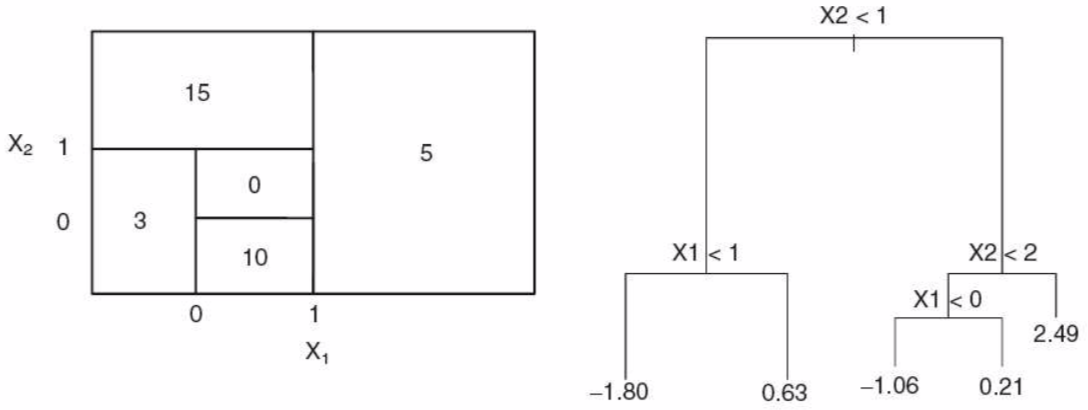
\includegraphics[width=4in]{fig}}
        \item Look at the tree in the right-hand panel of the same figure. Based on this tree, create a diagram similar to the left-hand panel of this figure. Divide the predictor space into the correct regions, and indicate the mean for each region.\\
       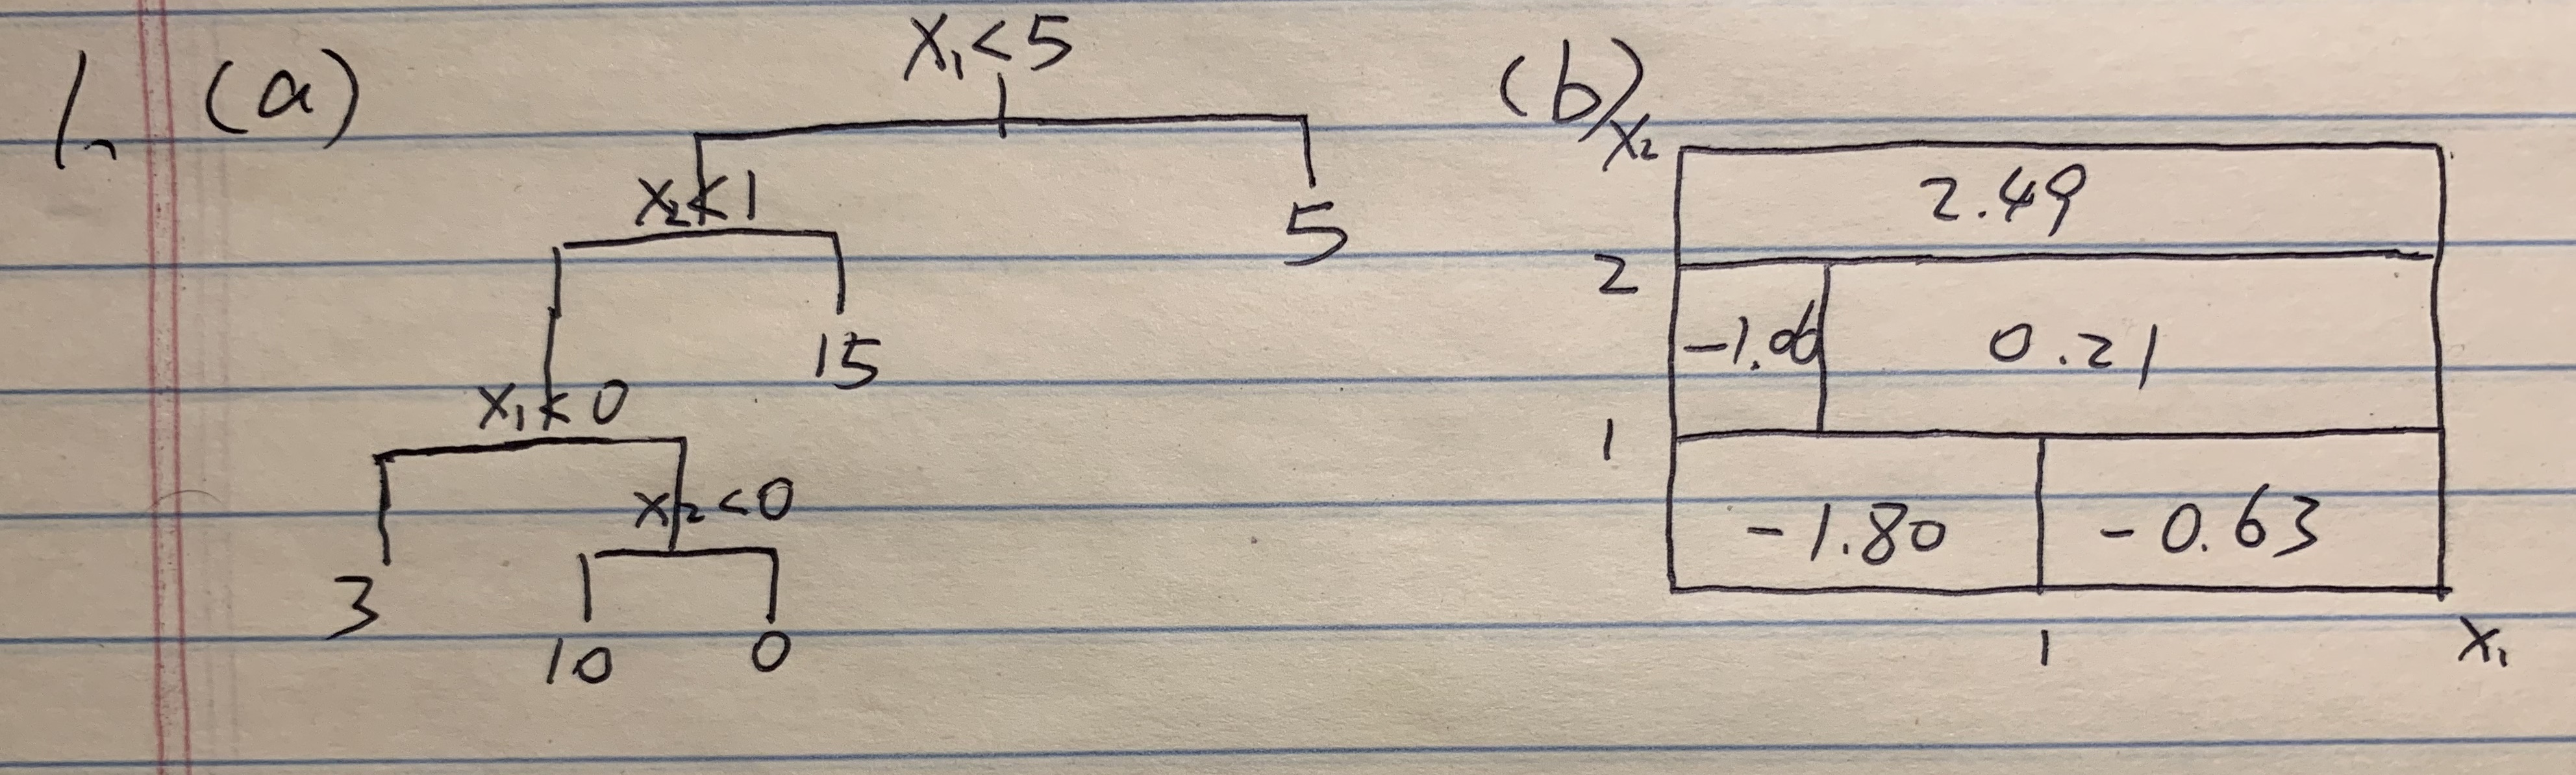
\includegraphics[width=15cm, height=3cm]{1}\\
	    \end{enumerate}
  % 2.
    \item \textbf{(Bagging; Chap. 8, \# 5, p. 332)} Suppose we produce ten bootstrapped samples from a data set containing red and green classes. We then apply a classification tree to each bootstrapped sample and, for a specific value of $X$, produce 10 estimates of $\boldsymbol{P}\{$Class is $\operatorname{Red} | X\} :$ 0.1, 0.15, 0.2, 0.2, 0.55, 0.6, 0.6, 0.65, 0.7, and 0.75.\\[10pt]
    There are two common ways to combine these results together into a single class prediction. One is the majority vote approach discussed in this chapter. The second approach is to classify based on the average probability. In this example, what is the final classification under each of these two approaches?
\begin{knitrout}
\definecolor{shadecolor}{rgb}{0.969, 0.969, 0.969}\color{fgcolor}\begin{kframe}
\begin{alltt}
\hlstd{p} \hlkwb{<-} \hlkwd{c}\hlstd{(}\hlnum{0.1}\hlstd{,} \hlnum{0.15}\hlstd{,} \hlnum{0.2}\hlstd{,} \hlnum{0.2}\hlstd{,} \hlnum{0.55}\hlstd{,} \hlnum{0.6}\hlstd{,} \hlnum{0.6}\hlstd{,} \hlnum{0.65}\hlstd{,} \hlnum{0.7}\hlstd{,} \hlnum{0.75}\hlstd{)}
  \hlcom{# majority vote approach}
\hlkwd{summary}\hlstd{(p}\hlopt{>}\hlnum{0.5}\hlstd{)}
\end{alltt}
\begin{verbatim}
##    Mode   FALSE    TRUE 
## logical       4       6
\end{verbatim}
\begin{alltt}
  \hlcom{# average probability}
\hlkwd{mean}\hlstd{(p)}
\end{alltt}
\begin{verbatim}
## [1] 0.45
\end{verbatim}
\end{kframe}
\end{knitrout}
    Under the majority vote approach, the classification would be red. Under the average probability approach, the classification would be green.
  % 3.
    \item \textbf{(Project; Chap. 8, \# 9, p. 334)}\\
    This problem involves the $\boldsymbol{OJ}$ (orange juice) data set which is part of the \texttt{ISLR} package. \texttt{library(ISLR)}; \texttt{attach(OJ)}; To find its description, type \texttt{?OJ}
      \begin{enumerate}[(a)]
      % a.
        \item Create a training set containing a random sample of 800 observations, and a test set containing the remaining observations.
\begin{knitrout}
\definecolor{shadecolor}{rgb}{0.969, 0.969, 0.969}\color{fgcolor}\begin{kframe}
\begin{alltt}
\hlkwd{set.seed}\hlstd{(}\hlnum{123}\hlstd{)}
\hlstd{n} \hlkwb{<-} \hlkwd{nrow}\hlstd{(OJ)}
\hlstd{train} \hlkwb{<-} \hlkwd{sample}\hlstd{(n,} \hlnum{800}\hlstd{)}
\end{alltt}
\end{kframe}
\end{knitrout}

      % b.
        \item Fit a tree to the training data, with Purchase as the response and the other variables except for Buy as predictors. Use the \texttt{summary()} function to produce summary statistics about the tree, and describe the results obtained. What is the training error rate? How many terminal nodes does the tree have?

\begin{knitrout}
\definecolor{shadecolor}{rgb}{0.969, 0.969, 0.969}\color{fgcolor}\begin{kframe}
\begin{alltt}
\hlstd{class.tree} \hlkwb{<-} \hlkwd{tree}\hlstd{(Purchase} \hlopt{~} \hlstd{.,} \hlkwc{data} \hlstd{= OJ[train,])}
\hlkwd{summary}\hlstd{(class.tree)}
\end{alltt}
\begin{verbatim}
## 
## Classification tree:
## tree(formula = Purchase ~ ., data = OJ[train, ])
## Variables actually used in tree construction:
## [1] "LoyalCH"   "PriceDiff" "SpecialCH" "PctDiscMM"
## Number of terminal nodes:  10 
## Residual mean deviance:  0.7289 = 575.8 / 790 
## Misclassification error rate: 0.1612 = 129 / 800
\end{verbatim}
\end{kframe}
\end{knitrout}
        The training error rate is 0.1612 and the number of terminal nodes is 10.
      % c.
        \item Type in the name of the tree object in order to get a detailed text output. Pick one of the terminal nodes, and interpret the information displayed.
\begin{knitrout}
\definecolor{shadecolor}{rgb}{0.969, 0.969, 0.969}\color{fgcolor}\begin{kframe}
\begin{alltt}
\hlstd{class.tree}
\end{alltt}
\begin{verbatim}
## node), split, n, deviance, yval, (yprob)
##       * denotes terminal node
## 
##  1) root 800 1073.000 CH ( 0.60500 0.39500 )  
##    2) LoyalCH < 0.482304 299  320.600 MM ( 0.22742 0.77258 )  
##      4) LoyalCH < 0.276142 172  127.600 MM ( 0.12209 0.87791 )  
##        8) LoyalCH < 0.0356415 56   10.030 MM ( 0.01786 0.98214 ) *
##        9) LoyalCH > 0.0356415 116  106.600 MM ( 0.17241 0.82759 ) *
##      5) LoyalCH > 0.276142 127  167.400 MM ( 0.37008 0.62992 )  
##       10) PriceDiff < 0.05 58   59.140 MM ( 0.20690 0.79310 )  
##         20) SpecialCH < 0.5 51   36.950 MM ( 0.11765 0.88235 ) *
##         21) SpecialCH > 0.5 7    5.742 CH ( 0.85714 0.14286 ) *
##       11) PriceDiff > 0.05 69   95.640 CH ( 0.50725 0.49275 ) *
##    3) LoyalCH > 0.482304 501  456.300 CH ( 0.83034 0.16966 )  
##      6) LoyalCH < 0.753545 236  292.000 CH ( 0.69068 0.30932 )  
##       12) PriceDiff < 0.265 147  202.300 CH ( 0.55102 0.44898 )  
##         24) PriceDiff < -0.165 40   47.050 MM ( 0.27500 0.72500 ) *
##         25) PriceDiff > -0.165 107  138.000 CH ( 0.65421 0.34579 )  
##           50) PctDiscMM < 0.10659 75  102.900 CH ( 0.56000 0.44000 ) *
##           51) PctDiscMM > 0.10659 32   24.110 CH ( 0.87500 0.12500 ) *
##       13) PriceDiff > 0.265 89   49.030 CH ( 0.92135 0.07865 ) *
##      7) LoyalCH > 0.753545 265   97.720 CH ( 0.95472 0.04528 ) *
\end{verbatim}
\end{kframe}
\end{knitrout}
        For node 8), if Customer brand loyalty for CH is less than 0.0356415, the observation will be classified to MM. The sample size of this box is 56, and the deviance for this node is 10.030. Also in this box, the proportion of MM is 0.98214, and that of CH is 0.01786.
      % d.
        \item Create a plot of the tree, and interpret the results.
\begin{knitrout}
\definecolor{shadecolor}{rgb}{0.969, 0.969, 0.969}\color{fgcolor}\begin{kframe}
\begin{alltt}
\hlkwd{plot}\hlstd{(class.tree)}
\hlkwd{text}\hlstd{(class.tree)}
\end{alltt}
\end{kframe}
\includegraphics[width=\maxwidth]{figure/3_d-1} 

\end{knitrout}
      % e.
        \item Predict the response on the test data, and produce a confusion matrix comparing the test labels to the predicted test labels. What is the test error rate?
\begin{knitrout}
\definecolor{shadecolor}{rgb}{0.969, 0.969, 0.969}\color{fgcolor}\begin{kframe}
\begin{alltt}
\hlstd{prediction} \hlkwb{<-} \hlkwd{predict}\hlstd{(class.tree,} \hlkwc{newdata} \hlstd{= OJ[}\hlopt{-}\hlstd{train,],} \hlkwc{type} \hlstd{=} \hlstr{"class"}\hlstd{)}
\hlkwd{table}\hlstd{(prediction,OJ}\hlopt{$}\hlstd{Purchase[}\hlopt{-}\hlstd{train])}
\end{alltt}
\begin{verbatim}
##           
## prediction  CH  MM
##         CH 158  37
##         MM  11  64
\end{verbatim}
\begin{alltt}
\hlkwd{mean}\hlstd{(prediction} \hlopt{!=} \hlstd{OJ}\hlopt{$}\hlstd{Purchase[}\hlopt{-}\hlstd{train])} \hlcom{# test error rate}
\end{alltt}
\begin{verbatim}
## [1] 0.1777778
\end{verbatim}
\end{kframe}
\end{knitrout}
        The test error rate is 0.1777778.
      % f.
        \item Apply the \texttt{cv.tree()} function to the training set in order to determine the optimal tree size.
\begin{knitrout}
\definecolor{shadecolor}{rgb}{0.969, 0.969, 0.969}\color{fgcolor}\begin{kframe}
\begin{alltt}
\hlstd{cv} \hlkwb{<-} \hlkwd{cv.tree}\hlstd{(class.tree,} \hlkwc{FUN} \hlstd{= prune.misclass )}
\end{alltt}
\end{kframe}
\end{knitrout}

      % g.
        \item Produce a plot with tree size on the x-axis and cross-validated classification error rate on the y-axis.
\begin{knitrout}
\definecolor{shadecolor}{rgb}{0.969, 0.969, 0.969}\color{fgcolor}\begin{kframe}
\begin{alltt}
\hlkwd{plot}\hlstd{(cv)}
\end{alltt}
\end{kframe}
\includegraphics[width=15cm]{figure/4_g-1} 

\end{knitrout}

      % h.
        \item Which tree size corresponds to the lowest cross-validated classification error rate?
\begin{knitrout}
\definecolor{shadecolor}{rgb}{0.969, 0.969, 0.969}\color{fgcolor}\begin{kframe}
\begin{alltt}
\hlstd{cv}\hlopt{$}\hlstd{size[}\hlkwd{which.min}\hlstd{(cv}\hlopt{$}\hlstd{dev)]}
\end{alltt}
\begin{verbatim}
## [1] 2
\end{verbatim}
\end{kframe}
\end{knitrout}
        The lowest cross-validated classification error rate is 2.
      % i.
        \item Produce a pruned tree corresponding to the optimal tree size obtained using cross-validation. If cross-validation does not lead to selection of a pruned tree, then create a pruned tree with five terminal nodes.
\begin{knitrout}
\definecolor{shadecolor}{rgb}{0.969, 0.969, 0.969}\color{fgcolor}\begin{kframe}
\begin{alltt}
\hlstd{tree.pruned} \hlkwb{<-} \hlkwd{prune.misclass}\hlstd{( class.tree,} \hlkwc{best}\hlstd{= cv}\hlopt{$}\hlstd{size[}\hlkwd{which.min}\hlstd{(cv}\hlopt{$}\hlstd{dev)] )}
\end{alltt}
\end{kframe}
\end{knitrout}

      % j.
        \item Compare the training error rates between the pruned and unpruned trees. Which is higher?
\begin{knitrout}
\definecolor{shadecolor}{rgb}{0.969, 0.969, 0.969}\color{fgcolor}\begin{kframe}
\begin{alltt}
\hlstd{train.pred} \hlkwb{<-} \hlkwd{predict}\hlstd{(class.tree,} \hlkwc{newdata} \hlstd{= OJ[train,],} \hlkwc{type} \hlstd{=} \hlstr{"class"}\hlstd{)}
\hlkwd{mean}\hlstd{(train.pred} \hlopt{!=} \hlstd{OJ}\hlopt{$}\hlstd{Purchase[train])} \hlcom{# train error rate}
\end{alltt}
\begin{verbatim}
## [1] 0.16125
\end{verbatim}
\begin{alltt}
\hlstd{train.pred.pruned} \hlkwb{<-} \hlkwd{predict}\hlstd{(tree.pruned,} \hlkwc{newdata} \hlstd{= OJ[train,],} \hlkwc{type} \hlstd{=} \hlstr{"class"}\hlstd{)}
\hlkwd{mean}\hlstd{(train.pred.pruned} \hlopt{!=} \hlstd{OJ}\hlopt{$}\hlstd{Purchase[train])} \hlcom{# train error rate. pruned}
\end{alltt}
\begin{verbatim}
## [1] 0.19125
\end{verbatim}
\end{kframe}
\end{knitrout}
        The training error rate of the pruned trees is higher.
      % k.
        \item Compare the test error rates between the pruned and unpruned trees. Which is higher?
\begin{knitrout}
\definecolor{shadecolor}{rgb}{0.969, 0.969, 0.969}\color{fgcolor}\begin{kframe}
\begin{alltt}
\hlstd{prediction.pruned} \hlkwb{<-} \hlkwd{predict}\hlstd{(tree.pruned,} \hlkwc{newdata} \hlstd{= OJ[}\hlopt{-}\hlstd{train,],} \hlkwc{type} \hlstd{=} \hlstr{"class"}\hlstd{)}
\hlkwd{mean}\hlstd{(prediction.pruned} \hlopt{!=} \hlstd{OJ}\hlopt{$}\hlstd{Purchase[}\hlopt{-}\hlstd{train])}
\end{alltt}
\begin{verbatim}
## [1] 0.1888889
\end{verbatim}
\end{kframe}
\end{knitrout}
        The test error rate of the pruned tree is $0.1888889 > 0.1777778$, the test error rate of pruned tree.
      \end{enumerate}
	\end{enumerate}
\end{document}
